\documentclass{article}

\usepackage[utf8]{inputenc}
\usepackage{graphicx}
\usepackage{geometry}
\usepackage{lmodern}
\usepackage{microtype}
\usepackage{fancyhdr}
\usepackage{hyperref}
\geometry{a4paper, margin=1in}

% en-têtes/pieds de page
\pagestyle{fancy}
\fancyhead[L]{Rapport de stage - OPT-NC}
\fancyhead[R]{Morgan CARRE}
\fancyfoot[C]{\thepage}


\begin{document}
	
	\begin{titlepage}
		\begin{center}
			{\LARGE \textbf{Rapport de Stage}} \\[1.5cm]
			{\large Effectué du \textbf{09/12/2024} au \textbf{[à déterminer]}} \\[1cm]
			
			
			
			{\large Réalisé au sein de la société :} \\[1cm]
			{\Large \textbf{DSI/GLIA OPT-NC}} \\[1cm]
			
			
\includegraphics[width=0.3\textwidth]{asset/logo_opt.jpg} \\[1cm] 
			
			
			\textbf{à Nouméa} \\[1cm]
			
			{\large \textbf{Développement d'une API REST des forfaits télécoms conteneurisée}} \\[1cm]
			
			{\large Présenté par :} \\[1cm]
			{\LARGE \textbf{Morgan CARRE}} \\[0.5cm]
			Étudiant en Licence Informatique, Semestre 5 \\[0.5cm]
			\textbf{Université de la Nouvelle-Calédonie} \\[0.5cm]
			
			
\includegraphics[width=0.2\textwidth]{asset/logo_universite.jpg} \\[2cm]
			
			{\large Supervisé par : \textbf{Adrien SALES}} \\[0.5cm]
		\end{center}
	\end{titlepage}
	\newpage
	\begin{abstract}
		Dans le cadre de mon stage à l'Université de la Nouvelle-Calédonie (UNC), en collaboration avec l'Office des Postes et Télécommunications de Nouvelle-Calédonie (OPT-NC) supervisé par Adrien SALES, j'ai travaillé sur le développement d'une API permettant de fournir des informations sur les différents forfaits télécoms. Ce projet a pour objectif de rendre les données publiques liées aux offres mobiles plus accessibles, en utilisant des outils modernes pour assurer une solution efficace et évolutive.
		
		L'API repose sur une stack technologique composée de Quarkus pour le développement de microservices performants, Flyway pour la gestion des migrations de base de données, et une base de données H2 pour le développement et les tests. 
		
		Ce rapport détaille les méthodologies adoptées, les technologies choisies et les différentes étapes de réalisation du projet, tout en mettant en lumière les défis rencontrés.
	\end{abstract}
	\newpage
	\tableofcontents
	%à compléter : titre et sous titres
	\newpage
	\section{Introduction}
	
	\subsection{Annonce du stage}
	
	Du \textbf{09 décembre 2024} au \textbf{[à déterminer]}, j’ai effectué un stage au sein de l’entreprise \textbf{OPT} (située à Nouméa, Nouvelle-Calédonie). Au cours de ce stage au département \textbf{DSI/GLIA (Direction des Systèmes d'Information / Gestion des Logiciels et Infrastructure Applicative)}, j’ai eu l’occasion de me plonger dans le développement d’une API permettant de fournir des informations sur les différents forfaits télécoms proposés par l’entreprise.
	
	Ce stage a été pour moi une opportunité d’explorer plusieurs aspects clés du métier de développeur \textbf{backend}, notamment en matière de gestion de bases de données, d’architecture de microservices, et de l’utilisation des technologies modernes comme Quarkus et Flyway. J’ai également pu développer des compétences techniques liées à la conception d’API REST.
	
	\subsection{Bref descriptif de l’entreprise et du déroulement du stage}
	
	L’Office des Postes et Télécommunications de Nouvelle-Calédonie (\textbf{OPT-NC}) est un acteur incontournable en Nouvelle-Calédonie, intervenant dans les domaines des télécommunications, de la finance, et des services postaux (et couvrant ainsi un large éventail de secteurs d'activité). L’entreprise propose des solutions variées allant des forfaits mobiles et connexions Internet aux services financiers et de distribution postale.
	
	Au sein de son département \textbf{DSI/GLIA}, j’ai intégré une équipe dynamique spécialisée dans le développement et la gestion de solutions logicielles.
	
	
	Supervisé par \textbf{Adrien SALES}, responsable au sein de l’équipe \textbf{GLIA}, j’ai bénéficié d’un encadrement rigoureux, favorisant l’apprentissage et la réalisation des différentes missions. Parmi ces missions, j’ai été chargé de concevoir une architecture basée sur Quarkus et Flyway, tout en suivant les bonnes pratiques de développement logiciel.
	
	\subsection{Problématique et objectifs du rapport}
	
	Ce stage m’a permis de contribuer au développement d’une API REST destinée à centraliser et rendre accessibles les informations sur les forfaits télécoms proposés par l’OPT-NC. L’objectif principal était de créer un outil moderne et fonctionnel, facilitant l’accès à ces données et leur utilisation dans d’éventuelles applications ou analyses.
	
	Ce rapport se concentre sur le processus de développement de l’API, en détaillant les étapes de conception, les choix technologiques réalisés, ainsi que les difficultés techniques rencontrées et les solutions mises en œuvre.
	
	\newpage
	\section{Méthodologie et outils}
	
	\subsection{Méthodologie de travail}
	
	Durant ce stage, j'ai suivi une approche de travail progressive, divisant le développement de l'API en plusieurs tâches spécifiques (appelées \textit{issues}). Chaque tâche correspondait à une fonctionnalité ou une étape précise du projet.
	
	Une fois une tâche terminée, je soumettais mon travail pour vérification à travers une demande spécifique appelée \textit{pull request}. Mon maître de stage, Adrien SALES, examinait ces propositions, identifiait d'éventuelles améliorations ou corrections, et me fournissait des retours. Après validation, les modifications étaient intégrées à la branche principale du projet, garantissant ainsi une progression structurée et contrôlée.
	
	Ce processus a été appliqué tout au long du projet pour assurer la qualité du code et une bonne gestion des étapes de développement.
	
	\subsection{Outils et technologies utilisés}
	
	Voici les principaux outils et technologies que j’ai utilisés pour ce projet :
\begin{itemize}
	\item \textbf{Java} : Langage de programmation principal utilisé pour le développement de l'API.
	\item \textbf{Maven} : Outil de gestion de projet et des dépendances.
	\item \textbf{Quarkus} : Framework Java pour le développement de microservices performants.
	\item \textbf{Flyway} : Outil de gestion des migrations de base de données, assurant la cohérence du schéma de données.
	\item \textbf{H2 Database} : Base de données embarquée utilisée pour les phases de développement et de test.
	\item \textbf{Git et GitHub} : Pour la gestion des versions et la collaboration.
	\item \textbf{Visual Studio Code} : Environnement de développement intégré.
	\item \textbf{HTTPie} : Outil en ligne de commande pour tester les endpoints de l'API.
	\item \textbf{Podman} : Outil pour la gestion et l'exécution de conteneurs, utilisé pour tester l'API en environnement conteneurisé.
	\item \textbf{Redocly} : Outil utilisé pour générer de la documentation statique à partir des spécifications OpenAPI.
\end{itemize}

	
	\section{Première tâche : conversion des sous-tâches en issues}
	
	La première tâche qui m’a été confiée au début de mon stage était de convertir une liste de sous-tâches fournies par mon maître de stage, Adrien SALES, en \textit{issues} distinctes sur \textbf{Github}. Cette démarche avait pour but de structurer et d’organiser les différentes étapes nécessaires à la réalisation de l’endpoint \texttt{/offres}, qui devait permettre de lister les types de forfaits, leurs pages de référence et une description associée.
	
	\subsection{Contexte}
	
	L’issue principale intitulée \textit{/offres : Lister les types d'abonnements \#1} décrivait les objectifs généraux et les actions attendues pour atteindre ce résultat. Voici les différentes sous-tâches qui devaient être transformées en issues individuelles :
	
	\begin{itemize}
		\item Étudier les données pour l'API \texttt{/offres} (\#4)
		\item nitialiser le projet Quarkus (\#5)
		\item Comprendre le rôle de Flyway
		\item Implémenter l'endpoint \texttt{/offres} avec Flyway
		\item Documenter avec des spécifications OpenAPI complètes
		\item Montrer un exemple d’appel avec \texttt{httpie}
		\item Implémentation au sein de Microcks (article à venir)
		\item Builder l’image en local avec \texttt{podman}
		\item Exécuter l’image en local avec \texttt{podman} et visualisation via [Podman Desktop](https://podman-desktop.io/)
		\item Générer la documentation OpenAPI
		\item Ajouter une CI pour tester le build Maven
		\item Mettre en œuvre des tests unitaires (seuil minimal 10\%)
		\item Lire des articles et regarder des vidéos sur l’automatisation de la documentation API avec GitHub, Redocly, et OpenAPI
		\item Générer une documentation HTML statique avec Redocly
		\item Livrer une première version du rapport au format \LaTeX{} : abstract et introduction
	\end{itemize}
	
	Pour illustrer la structuration et la mise en forme des issues, voici un exemple concret d’une issue que j’ai créée dans le cadre de cette tâche. Cela permet de visualiser comment chaque sous-tâche a été documentée et organisée pour garantir un suivi efficace.
	
	\begin{center}
		\textbf{Exemple d'issue mise en forme :}
	\end{center}
	
	\vspace{0.5cm}
	\begin{center}
		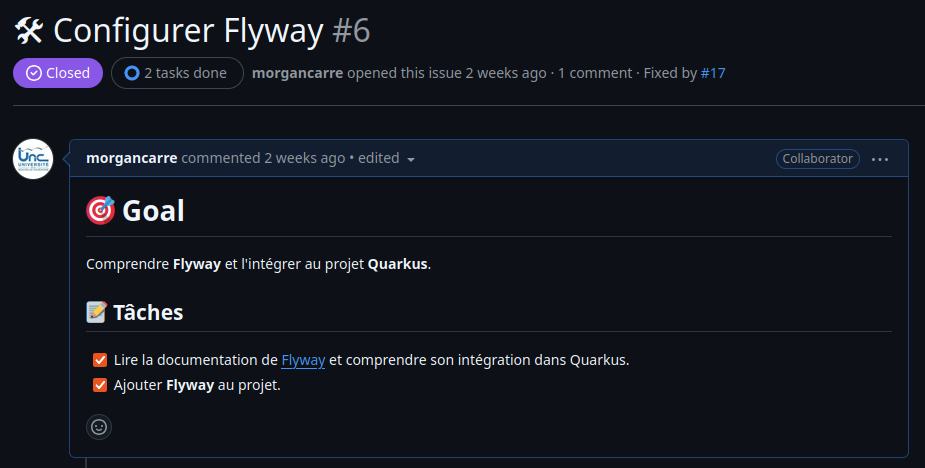
\includegraphics[width=0.8\textwidth]{asset/ex_issue.png}
	\end{center}
	
	Ce format inclut le titre de l’issue, une description détaillée des objectifs, et parfois des liens vers des ressources ou des outils nécessaires à sa réalisation.
	
	J’ai donc créé une issue distincte pour chaque sous-tâche, en précisant le contexte, les objectifs et les résultats attendus. Cette structuration a permis une meilleure visibilité sur les étapes du projet, tout en facilitant le suivi et la validation des différentes phases par mon maître de stage.
	\newpage
	\subsection{Identification des types de forfaits et création du fichier \texttt{offres.csv}}
	
	Ma deuxième tâche a consisté à identifier les différents types de forfaits disponibles sur la page de l’OPT intitulée \textit{"Identifiez le forfait qui vous ressemble"} (voir capture d’écran ci-dessous). Pour cela, j’ai analysé les caractéristiques propres à chaque forfait, notamment leur nom, leur description et leur utilisation, afin de les préparer sous une forme exploitable.
	
	\begin{figure}[h!]
		\centering
		
\includegraphics[width=0.8\textwidth]{asset/page_forfait.png}
		\caption{Page \textit{"Identifiez le forfait qui vous ressemble"} sur le site de l’OPT.}
		\label{fig:page_forfait}
	\end{figure}
	
	Après cette analyse, j’ai structuré ces informations dans un fichier au format \texttt{CSV}, nommé \texttt{offres.csv}. Ce fichier contient les champs suivants : l’identifiant (\texttt{id}), le nom (\texttt{desc}) et la description détaillée (\texttt{desc full}) de chaque forfait. Ce fichier est illustré dans la capture ci-dessous.
	
	\begin{figure}[h!]
		\centering
		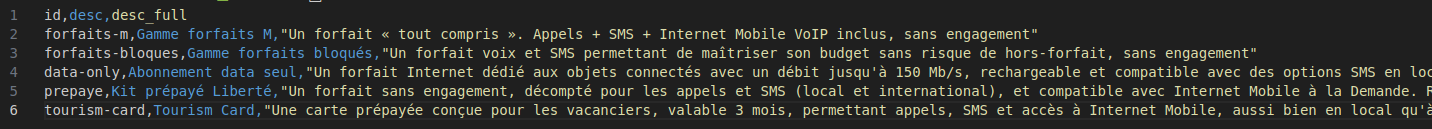
\includegraphics[width=0.8\textwidth]{asset/offres_csv.png}
		\caption{Extrait du fichier \texttt{offres.csv} contenant les données des forfaits.}
		\label{fig:offres_csv}
	\end{figure}
	
	J’ai choisi le format \texttt{CSV} en raison de sa portabilité et de sa facilité d’exploitation dans de nombreux cas. Ce format est particulièrement adapté à notre contexte, car il permet de charger efficacement les données dans une base de données à l’aide de Flyway, un outil utilisé pour gérer les migrations et remplir les tables avec les données préparées.
	
	\subsection{Initialisation du projet Quarkus et création d’un endpoint \textit{Hello World}}
	
	Une des premières étapes de mon projet a été d’initialiser le projet Quarkus et de mettre en place un endpoint basique permettant de tester le bon fonctionnement de l’environnement.
	
	\subsection{Initialisation du projet Quarkus et création d’un endpoint \textit{Hello World}}
	
	Une des premières étapes de mon projet a été d’initialiser le projet Quarkus et de mettre en place un endpoint basique permettant de tester le bon fonctionnement de l’environnement.
	
	\subsubsection{Initialisation du projet Quarkus}
	
	Pour initialiser le projet, j’ai utilisé la commande suivante :
	\begin{verbatim}
		mvn io.quarkus:quarkus-maven-plugin:create
	\end{verbatim}
	
	Cette commande a automatiquement généré la structure de base du projet, comprenant plusieurs fichiers et répertoires essentiels. Parmi les éléments les plus importants, on trouve :
	\begin{itemize}
		\item \texttt{pom.xml} : le fichier de configuration Maven qui liste les dépendances nécessaires au projet.
		\item \texttt{src/main/java} : le répertoire contenant le code source de l’application, avec un premier exemple de classe.
		\item \texttt{src/main/resources} : le répertoire pour les fichiers de configuration et les ressources statiques.
		\item \texttt{src/test/java} : le répertoire dédié aux tests unitaires.
	\end{itemize}
	
	Par défaut, Quarkus inclut un endpoint basique accessible à l’adresse \texttt{/hello}, qui renvoie un simple message \textit{"Hello World"}.
	
	\subsubsection{Lancement et test du projet}
	
	Pour exécuter le projet, il suffit d’utiliser la commande suivante :
	\begin{verbatim}
		mvn quarkus:dev
	\end{verbatim}
	
	Cette commande lance le projet en mode développement, avec un support pour le \textit{live coding}. Cela signifie que toutes les modifications apportées au code ou aux fichiers de configuration sont appliquées instantanément, sans besoin de redémarrer le serveur.
	
	Une fois lancé, le projet est accessible en local à l’adresse suivante :
	\begin{verbatim}
		http://localhost:8080
	\end{verbatim}
	
	J’ai ensuite vérifié le bon fonctionnement de l’endpoint par défaut \texttt{/hello} grâce à un appel réalisé avec l’outil HTTPIE. Voici une capture d’écran montrant la réponse renvoyée par le serveur :
	
	\begin{figure}[h!]
		\centering
		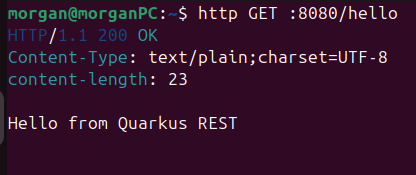
\includegraphics[width=0.8\textwidth]{asset/hello.png}
		\caption{Test de l'endpoint \texttt{/hello} avec HTTPIE.}
		\label{fig:hello_endpoint}
	\end{figure}
	
	\subsubsection{Avantages de Quarkus pour le développement}
	
	L’utilisation de Quarkus offre plusieurs avantages, notamment :
	\begin{itemize}
		\item Une structure de projet standardisée et prête à l’emploi, permettant de se concentrer rapidement sur le développement des fonctionnalités.
		\item Un mode développement interactif grâce à \textit{mvn quarkus:dev}, qui améliore la productivité.
		\item La possibilité d’ajouter facilement des extensions pour enrichir le projet, telles que Flyway ou Hibernate.
	\end{itemize}
	
	Cette première étape m’a permis de comprendre l’organisation d’un projet Quarkus et de mettre en place un environnement fonctionnel prêt à accueillir des fonctionnalités plus avancées.
	
	\subsection{Configuration de Flyway et mise en place de l'endpoint \texttt{/offres}}
	
	Dans le cadre de ce projet, il était nécessaire de centraliser les données des forfaits télécoms dans une base de données et de les exposer via un endpoint accessible. Pour ce faire, j'ai configuré Flyway pour gérer les migrations de base de données et j'ai développé l'endpoint \texttt{/offres} permettant de récupérer ces données.
	
	\subsubsection{Configuration de Flyway et de la base de données H2}
	
	La gestion des migrations de base de données a été confiée à Flyway, une solution reconnue pour son efficacité et sa simplicité d'intégration dans des projets modernes. Voici les principales étapes de configuration :
	
	\begin{itemize}
		\item Ajout des dépendances nécessaires dans le fichier \texttt{pom.xml} :
		\begin{itemize}
			\item \texttt{quarkus-flyway} : pour gérer les migrations de la base de données.
			\item \texttt{quarkus-jdbc-h2} : pour utiliser une base de données H2 en mémoire.
			\item \texttt{quarkus-hibernate-orm} : pour mapper les entités avec les tables de la base de données.
			\item \texttt{quarkus-resteasy-reactive-jackson} : pour gérer les réponses JSON dans les endpoints REST.
		\end{itemize}
		
		\item Configuration dans le fichier \texttt{application.properties} :
		\begin{verbatim}
			quarkus.datasource.db-kind=h2
			quarkus.datasource.jdbc.url=jdbc:h2:mem:forfaits-db;DB_CLOSE_DELAY=-1
			quarkus.datasource.username=admin
			quarkus.datasource.password=
			quarkus.flyway.migrate-at-start=true
			quarkus.flyway.locations=db/migration
		\end{verbatim}
		
		Ces paramètres définissent une base de données en mémoire H2, qui est initialisée à chaque démarrage de l'application et remplie  automatiquement grâce à Flyway.
		
		\item Création du fichier de migration \texttt{V1\_\_create\_and\_feed\_forfaits.sql} :
		Ce fichier SQL configure la table \texttt{Forfaits} et y insère les données issues du fichier \texttt{offres.csv} grâce à la méthode \texttt{CSVREAD}.
	\end{itemize}
	
	\subsubsection{Mise en place de l'endpoint \texttt{/offres}}
	
	L'endpoint \texttt{/offres} a été conçu pour exposer les données des forfaits télécoms sous forme JSON. Voici les étapes principales de son implémentation :
	
	\begin{itemize}
		\item Création de l'entité \texttt{Forfait}, mappée avec la table \texttt{Forfaits} dans la base de données. Cette classe représente la table \texttt{Forfaits} dans la base de données. Elle est annotée avec \texttt{@Entity}, indiquant à Hibernate qu'il s'agit d'une entité persistante. L'annotation \texttt{@Table(name = "Forfaits")} est utilisée pour spécifier explicitement le nom de la table dans la base de données. 
		
		Les champs \texttt{id}, \texttt{desc}, et \texttt{description} correspondent aux colonnes de la table \texttt{Forfaits}. L'annotation \texttt{@Id} sur le champ \texttt{id} désigne ce champ comme la clé primaire.
		
		Voici le code de l'entité \texttt{Forfait} :
		\begin{verbatim}
			@Entity
			@Table(name = "Forfaits")
			public class Forfait {
				@Id
				private String id;
				private String desc;
				private String description;
				
				// Getters et setters
				public String getId() {
					return id;
				}
				
				public void setId(String id) {
					this.id = id;
				}
				
				public String getDesc() {
					return desc;
				}
				
				public void setDesc(String desc) {
					this.desc = desc;
				}
				
				public String getDescription() {
					return description;
				}
				
				public void setDescription(String description) {
					this.description = description;
				}
			}
		\end{verbatim}
		
		Cette classe joue un rôle crucial, car elle permet de manipuler les données de la table \texttt{Forfaits} comme des objets Java.
		
		\item Développement de la ressource REST \texttt{OffresResource}, définissant l'endpoint \texttt{/offres}. Cette ressource utilise \texttt{EntityManager} pour exécuter une requête JPA récupérant toutes les données de la table.
	\end{itemize}
	
	Voici un extrait de la classe \texttt{OffresResource} :
	\begin{verbatim}
		@Path("/offres")
		@Produces(MediaType.APPLICATION_JSON)
		public class OffresResource {
			
			@Inject
			EntityManager entityManager;
			
			@GET
			public List<Forfait> getAllOffres() {
				return entityManager.createQuery("SELECT f FROM Forfait f", Forfait.class).getResultList();
			}
		}
	\end{verbatim}
	\newpage
	\subsubsection{Validation de l'endpoint avec HTTPIE}
	
	Pour vérifier le bon fonctionnement de l'endpoint \texttt{/offres}, un appel a été effectué à l'aide de l'outil HTTPIE. Voici une capture d'écran du résultat obtenu :
	
	\begin{figure}[h!]
		\centering
		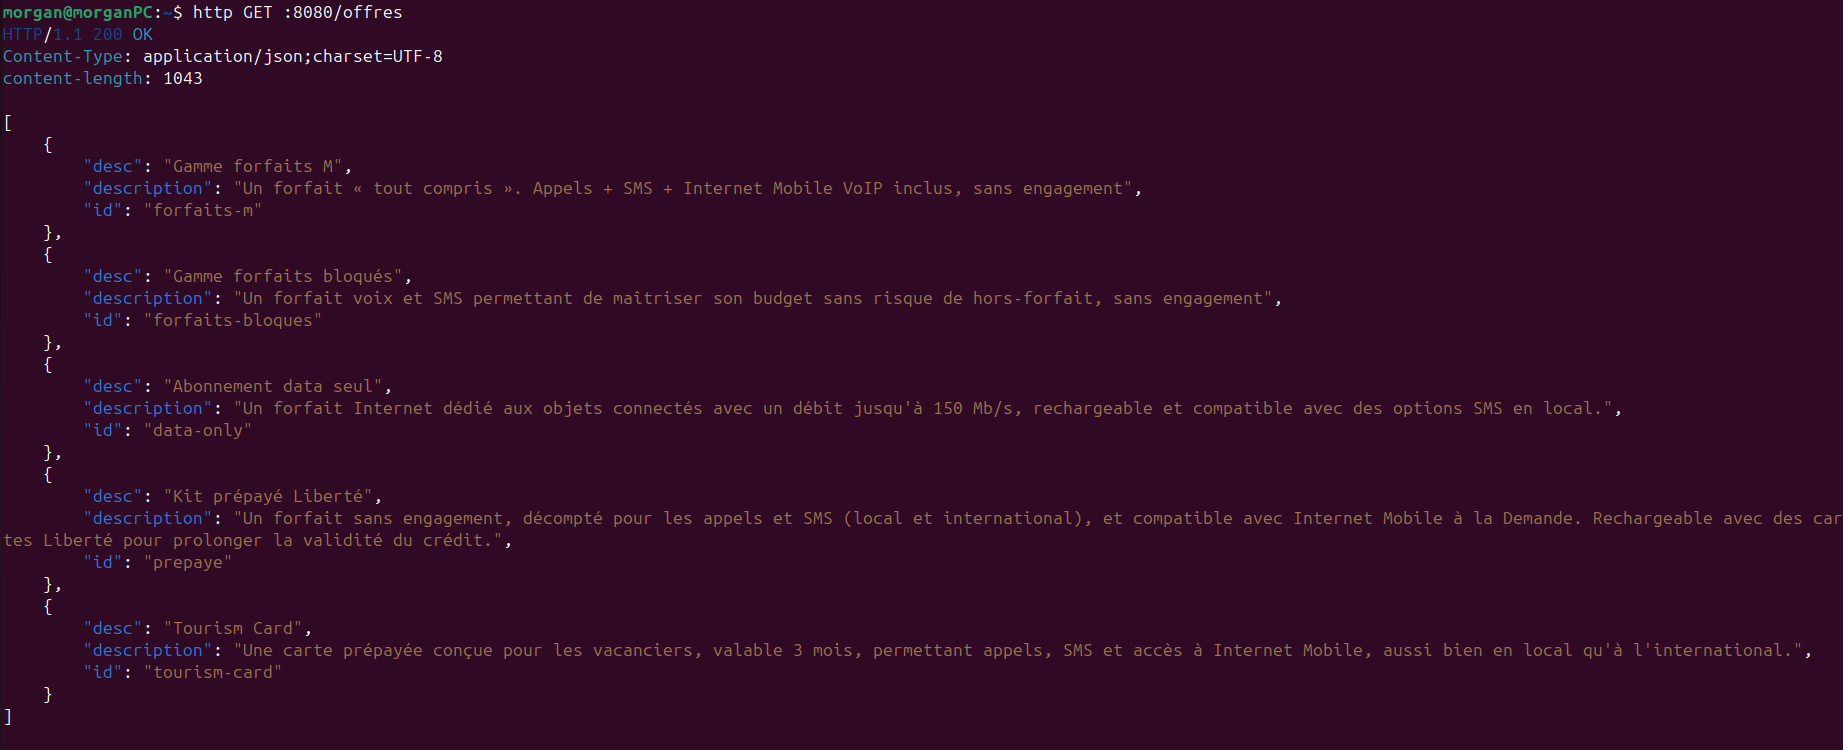
\includegraphics[width=1\textwidth]{asset/endpoint offres.png}
		\caption{Validation de l'endpoint \texttt{/offres} avec HTTPIE.}
		\label{fig:offres_endpoint}
	\end{figure}
	
\end{document}
